% arara: lualatex
% !TEX TS-program = LuaLaTeX


% https://phys.libretexts.org/TextBooks_and_TextMaps/College_Physics/Book%3A_College_Physics_(OpenStax)/03._Two-Dimensional_Kinematics/3.4%3A_Projectile_Motion

\documentclass{coderdojo}

\worksheet{7}{Monkey Wars}

\newcommand\contentsitem[2]{
	\item \hyperref[#1]{\color{section}\bfseries #2}
}

\usepackage{wrapfig}
\usepackage{float}

\newcommand\TODO[1]{
\begin{itemize}
\item[\todoSymbol] \color{todo} #1
\end{itemize}}


\newcommand\TEST[1][\bf Test your code!]{
	\centerline{\tikz\node[starburst, fill=yellow, draw=red, line width=2pt,align=center] {#1};}
}

\newcommand\TESTSMALL[2][\bf Test your code!]{
{\tikz[scale=#2]\node[starburst, fill=yellow, draw=red, line width=2pt,align=center] {#1};}
}


\begin{document}
\maketitle


\section*{Introduction}

\begin{exercise}[title=Monkey Wars]

\begin{minipage}{.5\textwidth}
\centerline {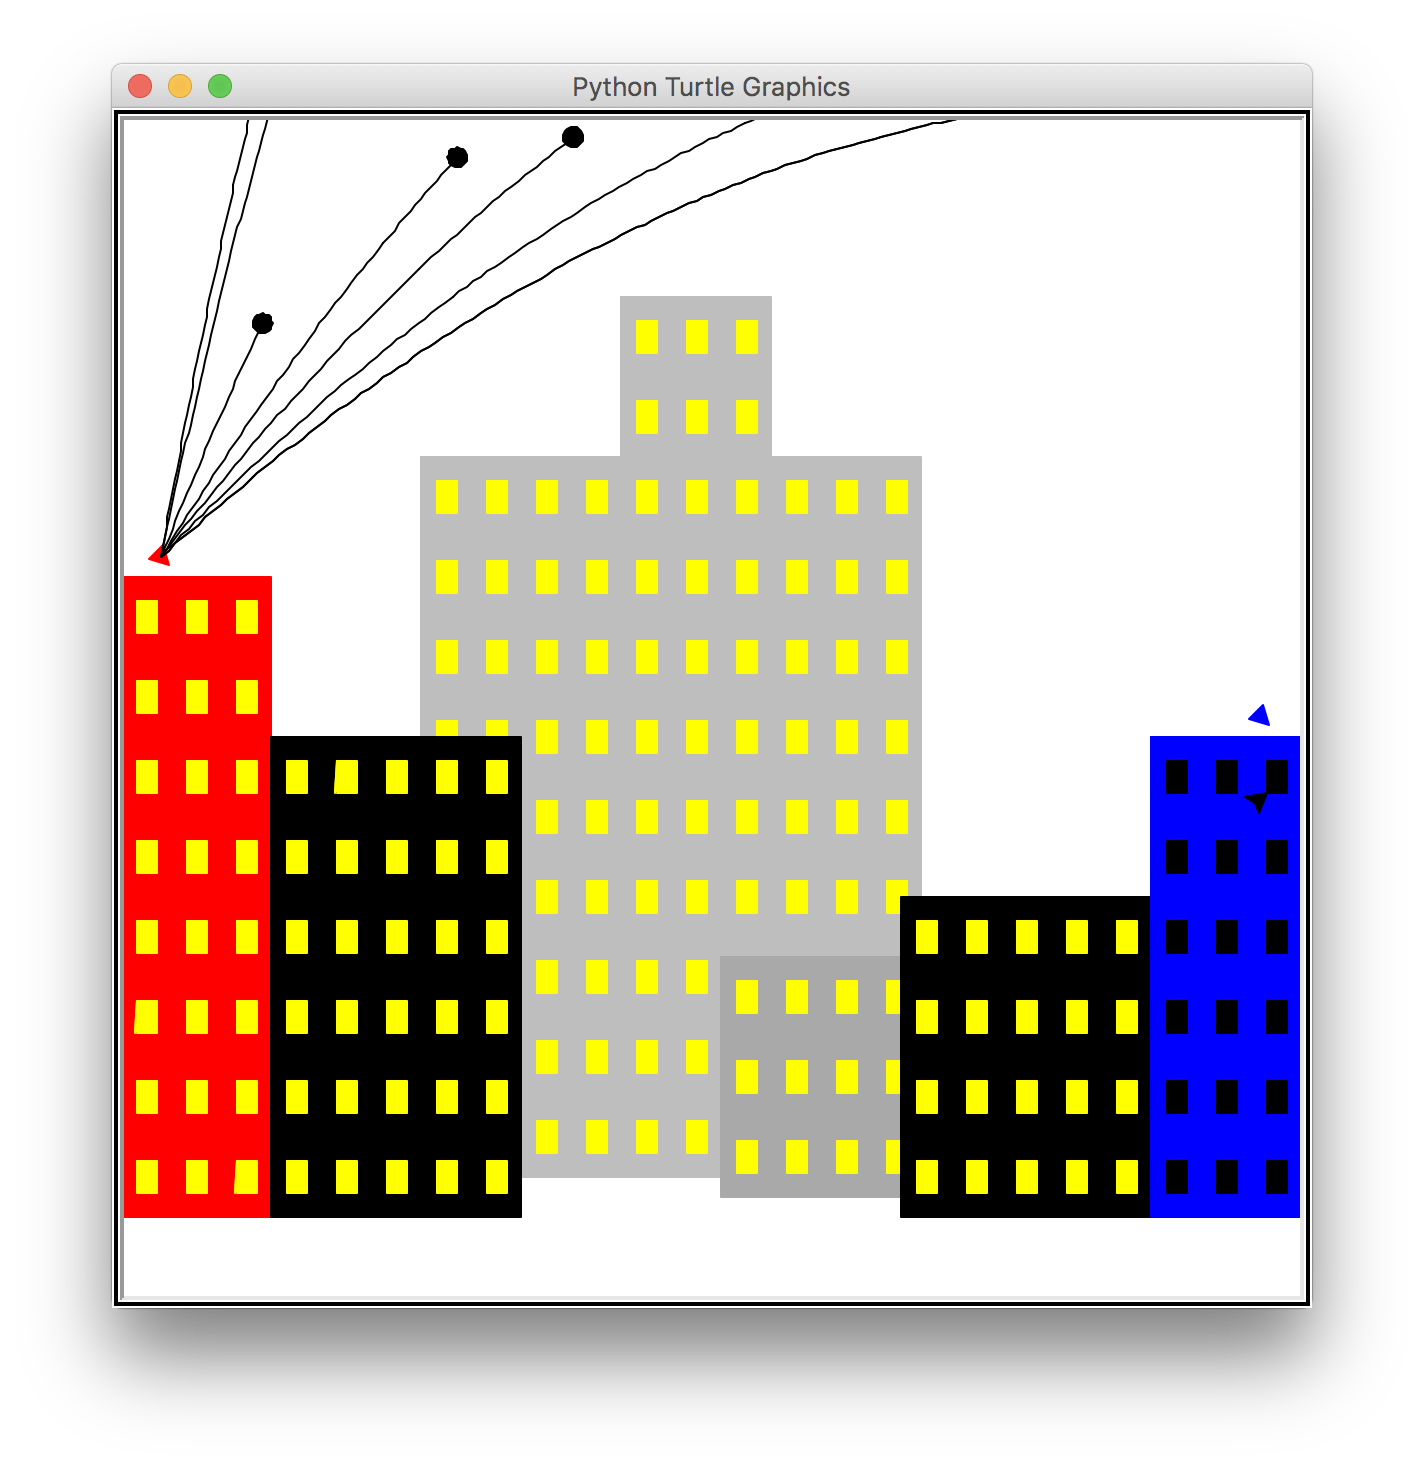
\includegraphics[width=.9\textwidth]{city}}
\end{minipage}
%
\begin{minipage}{.45\textwidth}

This is a very old arcade game, consisting of two monkeys on top of two skyscrapers throwing rocks at each other. 

Players race to aim and fire as quickly as possible to hit either the other player or the building that the other player is standing on.  As the building take damage the lights on the building go out. 
\end{minipage}

\end{exercise}

We are going to try something different today. I'm not going to give you any code --- well only a little code --- but instead I'm just going to say what I want the game to do and your job is to generate the code.  I expect you to get stuck in (many) places --- and would like you to ask each other and me, and hopefully we can work out the details together.

As before we have broken up the task in separate stages:

\begin{dingautolist}{192}

\contentsitem{city}{Design the city}

The city consists of:
\begin{itemize}
\item A red building on the left with random height of 2 to 10 floors and 3 windows wide.
\item A blue building on the right with random height of 2 to 10 floors and 3 windows wide.
\item Random building in between the red and blue building with taller building in the middle.
\end{itemize}


\contentsitem{physics}{The Players}

\begin{itemize}
\item
Draw two players on top of each building.
\item
We will create two turtles --- one for each player.

\end{itemize}


\contentsitem{physics}{Throwing Rocks}

\begin{itemize}
\item
To throw a rock we are going to use our projectile motion code from two weeks ago.
\end{itemize}


\end{dingautolist}


%%%%%%%%%%%%%%%%

\section{Design the City}\label{sec:city}

Creating the city will take us some time, and to simplify development we will change some of the default \code{turtle} settings.

\TODO{Create file called \code{city.py} and insert the following code.}

\codeonly{title={\code{Monkey_Wars.py}}}{1}{12}{code}{Monkey_Wars.py}  

This code
\begin{itemize}
\item Loads in libraries that we will need.
\item[(line 5)] Creates a screen in which the turtles can move and draw.
\item[(line 6)] Moves the screen to the top left of the computer screen (so hopefully it won't be displayed on top of your code).
\item[(line 7)] Changes the coordinates of the screen so that the bottom left corner is $(-300,-10)$ and the top right corner is $(300,500)$. This will make drawing of the building easier.
\item 
In lines 9 and 10 we create variables that control the height and width of buildings.
\item[(line 12)] 
Finally we create our hard working turtle, \code{bob}.

\end{itemize}


\TODO{Write a function that draws a filled rectangle at a given location}
 
\codeonly{}{21}{21}{code}{Monkey_Wars.py}  

Now to draw a building we need to specify:
\begin{itemize}
\item The position of the building --- we will use the bottom left corner as the anchor point.
\item The height in number of floors.
\item The width in number of windows in each floor.
\item The colour --- defaults to \code{black}.
\item And draw in the windows (in \code{yellow}).
\end{itemize}
So we can draw a building by just drawing rectangles ---  so we will use function \code{draw_rectangle} for all drawings. 

\clearpage
\TODO{Write a function that draws a building using the following line.}

\codeonly{}{40}{40}{code}{Monkey_Wars.py}  

This should draw a building with default colour of \code{black} consisting of \code{floors} floors and \code{windows} windows per floor.

\begin{center}
\begin{tcolorbox}[width=.9\textwidth,title=What does the parameter \code{health} do?]
I want to use the parameter \code{health} to represent the health of the building and to control how many lights as the building sustains more damage.  We will talk how this can be implemented during the session.
\end{tcolorbox}
\end{center}

\TODO{Write a function that draws the city using the following code. The 
\code{screen.tracer(0)} line allows the city to be drawn before displaying it.}

\codeonly{}{15}{18}{code}{scraps.py}  


\section{The Players}

\TODO{The first stage of the game is done, so it is a good idea to save this and continue to work on the game using a different file --- save your code and change the file name to \code{players.py}}

The players are both turtles --- lets called them \code{red} and \code{blue} so we write 

\codeonly{}{13}{14}{code}{Monkey_Wars.py}  

\begin{itemize}
\item 
Place the players on top of their buildings:
\begin{itemize}
\item So we need to remember how tall both the red and blue building are! Go back to your \code{draw_city} function and see where you generated a random number for the height of each building.  Save those values to \code{red.floors} and \code{blue.floors}.
\end{itemize}
\item 
Point both players (turtles) facing up --- so if they fire they will damage their own building!
\item
Add event listeners so that ``\code{q}" and ``\code{a}" and used to aim the red player, and ``\code{,}" and ``\code{.}" --- these are the ``\code{<}'' and ``\code{>}''' keys --- are used to aim the blue player.  
\begin{itemize}
\item The event listening code is the same as we used in the Graphical Take Away game, so look over previous worksheets if --- horror of horrors --- you have forgotten anything. 
\end{itemize}
\item
Add events listeners so that ``\code{z}'' and ``\code{m}'' fire the red and blue player rocks --- to avoid duplicate code we are going to have a single fire function for both players as shown in the following code.
\end{itemize}

\TODO{Insert the following functions into your program and verify that the key events work as expected. You need a function \code{fire(player)} to check if your code works at this point.}

\codeonly{}{93}{116}{code}{Monkey_Wars.py}  

% TODO include code up to 118 and add more detail to get pages 5 and 6 -- not done now due to time.

\section{Throwing Rocks}

Next we need to deal with the rocks flying through the air! This has some tricky bits so I'm not going to do this here but talk about it in the sessions.

\TODO{Write the skeleton of the function \code{fire} as given below and we will fill in the details in the session.}

\codeonly{}{1}{14}{code}{scraps.py}  

\end{document}
















In worksheet 2 we developed the {\em Take Away Game} and we started in worksheet 3 with a graphical version of this game. We covered the various building blocks need for this but we never got to build the actual game. Lets try to get that completed today.

\begin{figure}[H]
\begin{minipage}{.5\textwidth}
\begin{exercise}
Game consists of a pile of coins with two players taking turns to play. At each turn the player decides to take 1, 2 or 3 coins.  The player who take the last coin wins.

\centerline {\includegraphics[page=12]{take_away_game}}
\end{exercise}
\end{minipage}
\begin{minipage}{.5\textwidth}
\centerline {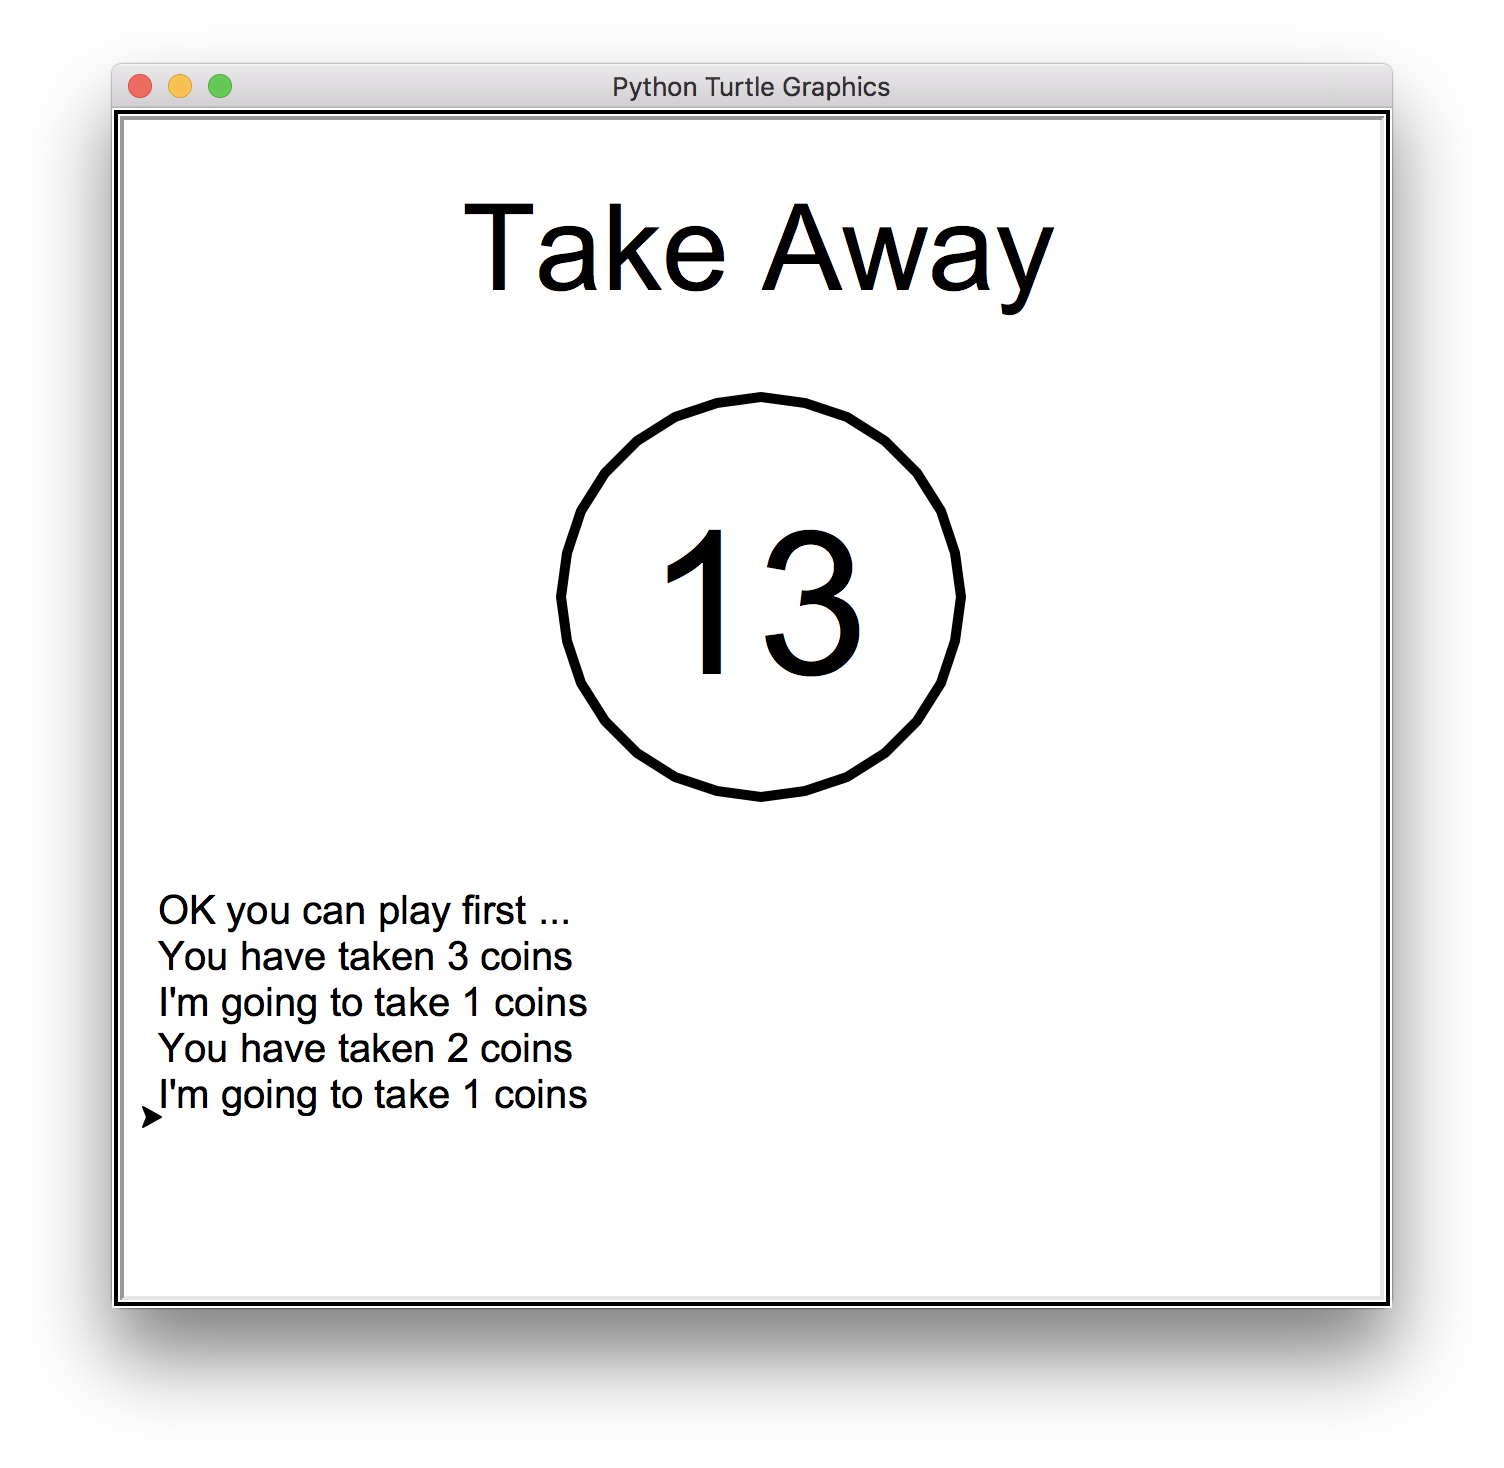
\includegraphics[width=.8\textwidth]{Completed_Game.png}}
\end{minipage}
\caption{Description of game and output from graphical implementation.}
\end{figure}

\vspace{12pt}
This will be one of the longest programs we will have written so far, and we will need to use the ideas from earlier worksheets so be prepared to look over the earlier worksheets!

As before we have broken up the task in separate stages:

\begin{dingautolist}{192}

\contentsitem{physics}{Events --- We do Nothing unless Prompted!}

Remember back in worksheet 3, we talked about {\em Event Programming}. In event programming we give the computer a set of instructions that look like 

\centerline{``If THIS happens, then do THAT''}

Where, for us the THIS will be various keys being pressed.

\contentsitem{drop}{States --- Writing Programs that are Moody}

When an event occurs our program may need to do different things depending on what is happening with rest of the programs. We mange this using states.

\contentsitem{drop}{Tying it all Together}

Next we will implement the game.

\contentsitem{drop}{Implementing the GUI}

Finally!! we get to the long awaited and overdue graphics !!

\end{dingautolist}

\clearpage

\section{Events --- We do Nothing unless Prompted!}

\TODO{Create a new file called \code{Events.py} and insert the following code.

\TODO{Save your \code{Events.py} as \code{TakeAway_Graphical_Events.py} and modify it so that it responds to all of the required events as follows.}

Run code and see what happens \ldots}

\codeandoutput{title={\code{Events.py}}}{1}{20}{code}{Events.py}{

	\centering	
	\tikz\node[fill=white]{
	
\includegraphics[clip,trim=0 10 0 10, width=\textwidth]{code/Events.pdf}};
}

It is boring right?  Noting happens, the computer just sits there waiting and waiting and waiting \ldots

So what is the code doing?
\begin{itemize}
\item
In lines 1 to 3, we import the \code{turtle} library and create a screen for our turtle to run around in and create a turtle, which we call \code{bob}.
\item
In lines 6 and 7, we define a simple function that, for now, just outputs a message.
\item
In line 9 is where the magic happens.  Here we tell the screen that if it should ``hear'' the key ``s'' being pressed then it should stop whatever it was doing and start running the code in function \code{startGame}.

\item
Finally in line 11, we tell the screen to start listening --- so it has no excuse if it does not respond to me pressing the ``s'' key now! 
\end{itemize}

\TODO{Create a new file called \code{Events.py} and insert the following code.

\begin{itemize}
\item
Run the above code and press ``s'' a few times. What happens?
\item
What happens if you press other keys?
\item
What happens if you press ``S''?  

Fix the program so that it will also output message when user presses ``S''.

\end{itemize}}

Ok now that we are happy with how events are programmed, we need to think about what events we will need for our game:

\begin{itemize}
\item During the game we need to listen out for keys ``1'', ``2'', and ``3'' begin pressed --- they will represent the number of coins the player wants to remove.
\item Also it would be nice if we could start a new at any point --- we will use ``s'' for that (as in our first program above).
\item Finally to implement an idea that I stole from Amy, it would be nice at the start of the game to ask the player if they wanted to go first or second.  So we need to listen for events ``n'' and ``y'' also. 
\end{itemize}


\TODO{Save your \code{Events.py} as \code{TakeAway_Graphical_Events.py} and modify it so that it responds to all of the required events as follows.}

\codeonly{title={\code{TakeAway_Graphical_Events.py}}}{1}{100}{code}{TakeAway_Graphical_Events.py}  


\TODO{Verify that the above code does respond to each of the required events and can handle both upper and lower case input.}


OK, so where are we now \ldots\ we have got a program that responds to events --- I admit the response is a bit sad, but it is a start --- however we do not want our programs to always give the same response to an event.  We need our program to be moody!  This is the focus of the next section.

\vfill

\parbox{5.6cm}{\TESTSMALL[Test your code!]{0.2}}\parbox{11cm}{
As our program gets more complicated, bugs will be harder to find.
It is vital you test your code at each step of development.}

\vfill

\clearpage
\section{States --- Writing Programs that are Moody}

If we run through in our heads what playing the game would be like we would end up with something like the following structure

\begin{description}
\item[start] Game board is setup and game is about to start.
\begin{itemize}
\item
Program has asked the player if they want to go first.  Currently waiting for an ``Y'' or ``N'' event, all other events are ignored.

\end{itemize}
\item[human] Playing the game and waiting for human move.
\begin{itemize}
\item  waiting for human move so events ``1'', ``2'' or ``3''.  
\item Also allowed is ``s'' to start a new game.
\end{itemize}
\item[computer] Playing game and computer is calculating its move. 
\item[end] Game is over (all coins taken).
\begin{itemize}
\item Only valid event is ``s'' to start a new game.
\end{itemize}
\end{description}

% TO DO -- put this into a table with events as columns and states as rows

Listing the states is useful but we find diagrams easier to follow so would take the above information and build a diagram like the following

\begin{figure}[H]\centering
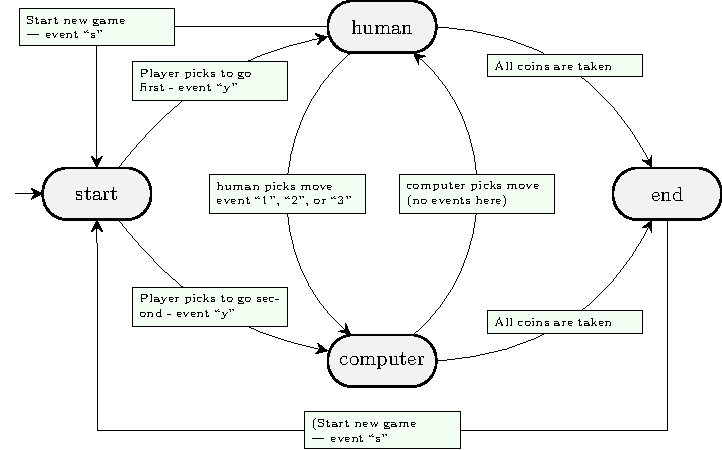
\includegraphics[width=\textwidth]{states}
\caption{State and event diagram of game --- ``what to listen out for and when''.}
\end{figure}

The above diagram is missing some details --- which we will discuss soon --- but we can start coding our game based on this now.
\clearpage
\TODO{Save your \code{TakeAway_Graphical_Events.py} as \code{TakeAway_Graphical_States.py} and modify it so that it matches the following code.}

\codeonly{title={\code{TakeAway_Graphical_States.py}}}{1}{100}{code}{TakeAway_Graphical_States.py}  

So what does the above code do?

\begin{itemize}
\item
In line 5, we store the state in our turtle \code{bob}.

\item
We can press ``s'' at any time to start a new game, then state switches to {\bf start}.
\item
When {\bf and only when} we are in {\bf start} state we can press ``y'' or ``n'' to select going first or second.
\item
When in state {\bf human} we can press ``1'', ``2'' or ``3'' to make a move.  
\end{itemize}

Next we need to start filling in the logic within each state\ldots
\clearpage

\subsection{Implementing State: start}

When a player presses ``s'' to start a new game what should happen?
\begin{enumerate}
\item
Pick a random number of coins, say in range $15\ldots21$, to start game.

We will store the number of coins in our turtle \code{bob}.
\item
Output message, saying number of coins.
 \item
Switch state to {\bf start} and wait for events ``n'' and ``y''. 
\end{enumerate}

\TODO{Save your \code{TakeAway_Graphical_States.py} as \code{TakeAway_Graphical_Basic.py} and modify it as follows.

We want to generate random numbers so  we import the \code{random} library, by inserting line 

\codeonly{}{2}{2}{code}{TakeAway_Graphical_Basic.py}  

Change function \code{startGame} to 

\codeonly{}{8}{12}{code}{TakeAway_Graphical_Basic.py}  
}

\parbox{3cm}{\TESTSMALL[Test!]{0.2}}\parbox{14cm}{
At this point if you press ``s'' to start a new game, then press you should get a message sayin the initial number of coins.}

\subsection{Implementing State: human}

We have three events to deal with --- ``1'', ``2'' and ``3'' --- and their linked functions. But all three events will have similar behaviour so to avoid duplicate code we write a single function that the three linked functions point to 

\TODO{Modify your \code{TakeAway_Graphical_Basic.py} to:

\codeonly{}{25}{37}{code}{TakeAway_Graphical_Basic.py}  
}

\parbox{3cm}{\TESTSMALL[Test!]{0.2}}\parbox{14cm}{
At this point if you press ``s'' to start a new game, then press ``y'' to move first, then you can pick ``1'', ``2'', or ``3'' to play.}

\subsection{Implementing State: computer}

In earlier worksheets we have covered the logic to get the computer to  
\begin{itemize}
\item play as a naive player --- just taking a random number of coins.
\item playing with optimal strategy
\item playing with a skill level, that can be set to any values between zero (for naive player) up to one (for optimal player).  
\end{itemize}
So here we will start with the naive player and leave that more fancy strategies as an exercise.

\TODO{Insert the following function into your \code{TakeAway_Graphical_Basic.py}

\codeonly{}{40}{44}{code}{TakeAway_Graphical_Basic.py}  
}

We can't test this function yet because we are missing a {\bf glue} function that monitors the overall state of the game

\subsection{Linking the stages --- functions update}

\TODO{Insert the following function into your \code{TakeAway_Graphical_Basic.py}

\codeonly{}{47}{64}{code}{TakeAway_Graphical_Basic.py}  

And at bottom of functions \code{startGame}, \code{humanMove}, \code{computerMove}, \code{player_No}, and \code{player_Yes} append line

\codeonly{}{13}{13}{code}{TakeAway_Graphical_Basic.py}  
}

\subsection{Implementing Graphics --- function drawScreen}

Currently our program won't run since we call function \code{drawScreen} which we have not yet defined.

\TODO{Fix that issue by inserting the function 

\codeonly{}{66}{67}{code}{TakeAway_Graphical_Basic.py}  

}

\parbox{3cm}{\TESTSMALL[Test!]{0.2}}\parbox{14cm}{
At this point if you press ``s'' to start a new game, you can play the game. There is no graphics and all message are displayed at the console.}

\TODO{Now to build up our graphics we replace the above function with the following 

\codeonly{}{66}{90}{code}{TakeAway_Graphical_Complete.py}  

Also to get the messages displayed on the graphical screen, instead of the console, we need to make the following changes:

\ding{43}$\quad$ In function \code{startGame} change line 
\codeonly{}{10}{10}{code}{TakeAway_Graphical_Basic.py}  
to
\codeonly{}{10}{10}{code}{TakeAway_Graphical_Complete.py}  

\ding{43}$\quad$ In the rest of program change any \code{print} line like 
\codeonly{}{11}{11}{code}{TakeAway_Graphical_Basic.py}  
to 
\codeonly{}{11}{11}{code}{TakeAway_Graphical_Complete.py}  

You will need to do this in eight places!
}


\parbox{3cm}{\TESTSMALL[Test!]{0.2}}\parbox{14cm}{
Finally we have a finished product.  Test, Test and Test!}

\clearpage
\section{Exercises (or no rest for the wicked)}

The current game is pretty good --- even if I say so myself --- but it has issues.  Your job is to fix the problems and make me look good!

\begin{enumerate}
\item 
You have to press ``s'' to start playing the game. Fix this by inserting code 

\codeonly{}{76}{76}{code}{TakeAway_Graphical_Basic.py}  

just before line 

\codeonly{}{77}{77}{code}{TakeAway_Graphical_Basic.py}  

\item
The computer strategy is just to pick randomly. Improve on this.

\item
The human player can always take up to three coins, regardless of how many coins are left.  This needs to be fixed.

\item 
It would be nice to add a confirmation question in response to a ``s'' pressed event that occurs during a game, i.e., when state is {\bf human} or {\bf computer}.
\end{enumerate}
\end{document}














